% Fig 1 - JEPA architecture for vortex-jepa manuscript.
%
% UNCONDITIONED model: no gust parameters enter the encoder or the predictor.
% The c=(G,D,Y) -> predictor arrow and the AdaLN-Zero conditioning have been
% removed; the predictor advances the latent from its own history alone.
%
% Layout (v6): losses placed NEXT to their targets so arrows are short
% and never cross other boxes.
%   CENTER:            input -> encoder -> z_t -> predictor -> zhat -> decoder -> xhat
%
% Standalone-compilable: pdflatex fig1_jepa_architecture.tex

\documentclass[border=10pt,tikz]{standalone}
\usepackage{tikz}
\usepackage{amsmath,amssymb}
\usetikzlibrary{positioning,arrows.meta,fit,shapes.geometric,calc,backgrounds}

\begin{document}

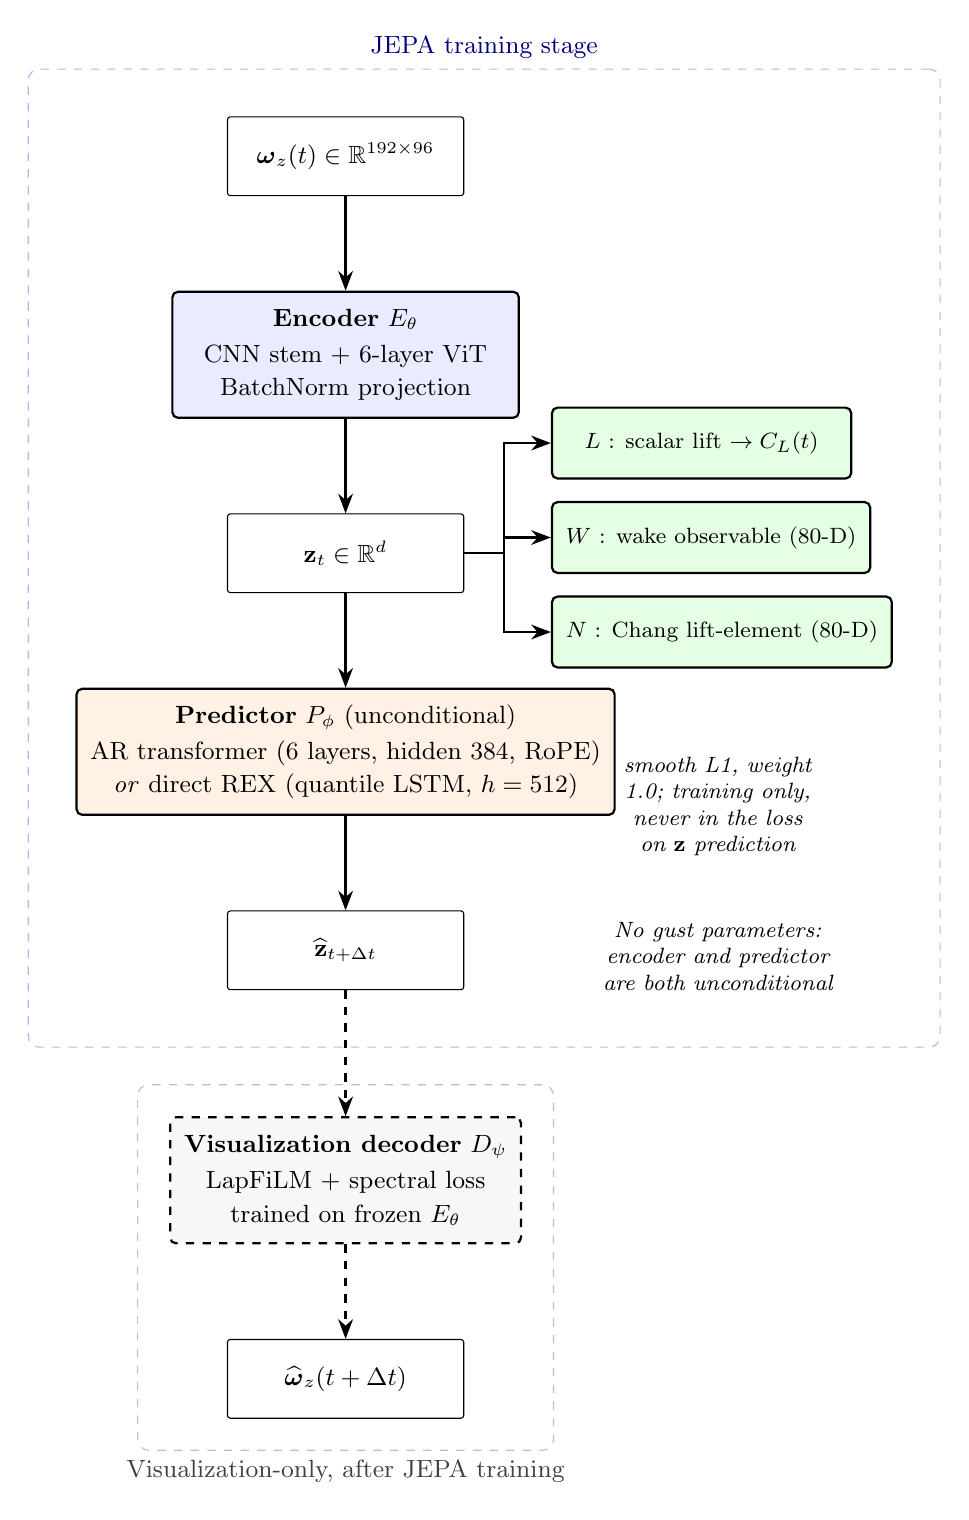
\begin{tikzpicture}[
    font=\small,
    box/.style={draw, rounded corners=2pt, align=center, inner sep=5pt, thick},
    encoder/.style={box, fill=blue!8,    minimum width=44mm, minimum height=16mm},
    predictor/.style={box, fill=orange!10, minimum width=56mm, minimum height=16mm},
    decoder/.style={box, fill=gray!6, dashed, minimum width=44mm, minimum height=16mm},
    obs/.style={box, fill=green!10, minimum width=38mm, minimum height=13mm,
                font=\footnotesize},
    state/.style={draw, rectangle, rounded corners=1pt, fill=white,
                  minimum height=10mm, minimum width=30mm, inner sep=3pt},
    cond/.style={box, fill=yellow!18, minimum width=38mm, minimum height=14mm,
                 font=\footnotesize},
    loss/.style={draw, rectangle, dashed, fill=red!5, inner sep=4pt,
                 minimum height=12mm, minimum width=46mm, align=center,
                 font=\footnotesize},
    arr/.style={-{Stealth[length=2.5mm]}, thick},
    lossarr/.style={-{Stealth[length=2mm]}, dashed, semithick, red!70!black}
  ]

  % ===== central spine =====
  \node[state] (input) {$\boldsymbol{\omega}_z(t) \in \mathbb{R}^{192 \times 96}$};
  \node[encoder, below=12mm of input] (enc)
    {\textbf{Encoder} $E_{\theta}$ \\[2pt]
     CNN stem $+$ 6-layer ViT \\[1pt]
     BatchNorm projection};
  \node[state, below=12mm of enc] (zt) {$\mathbf{z}_t \in \mathbb{R}^{d}$};
  \node[predictor, below=12mm of zt] (pred)
    {\textbf{Predictor} $P_{\phi}$ (unconditional) \\[2pt]
     AR transformer (6 layers, hidden 384, RoPE) \\[1pt]
     \emph{or} direct REX (quantile LSTM, $h = 512$)};
  \node[state, below=12mm of pred] (zhat) {$\widehat{\mathbf{z}}_{t+\Delta t}$};
  \node[decoder, below=16mm of zhat] (dec)
    {\textbf{Visualization decoder} $D_{\psi}$ \\[2pt]
     LapFiLM $+$ spectral loss \\[1pt]
     trained on frozen $E_{\theta}$};
  \node[state, below=12mm of dec] (xhat)
    {$\widehat{\boldsymbol{\omega}}_z(t + \Delta t)$};

  \draw[arr] (input) -- (enc);
  \draw[arr] (enc) -- (zt);
  \draw[arr] (zt) -- (pred);
  \draw[arr] (pred) -- (zhat);
  \draw[arr, dashed] (zhat) -- (dec);
  \draw[arr, dashed] (dec)  -- (xhat);

  % ===== supervision heads (training only), branching off z_t =====
  % West-anchored so the differing box widths never protrude toward the
  % spine; the stack sits fully clear of the predictor's right edge.
  \node[obs, anchor=west, minimum height=9mm] (headL)
    at ($(zt.east)+(11mm,14mm)$) {$L$ : scalar lift $\rightarrow C_L(t)$};
  \node[obs, anchor=west, minimum height=9mm] (headW)
    at ($(zt.east)+(11mm,2mm)$) {$W$ : wake observable ($80$-D)};
  \node[obs, anchor=west, minimum height=9mm] (headN)
    at ($(zt.east)+(11mm,-10mm)$) {$N$ : Chang lift-element ($80$-D)};
  \node[align=center, font=\footnotesize\itshape, text width=42mm,
        below=10mm of headN.south east, anchor=north east]
    (headnote) {smooth L1, weight 1.0; training only, \\
                never in the loss on $\mathbf{z}$ prediction};
  \draw[arr] (zt.east) -- ++(5mm,0) |- (headL.west);
  \draw[arr] (zt.east) -- ++(5mm,0) |- (headW.west);
  \draw[arr] (zt.east) -- ++(5mm,0) |- (headN.west);

  % ===== unconditional predictor: no gust parameters enter the model =====
  \node[align=center, font=\footnotesize\itshape, text width=34mm,
        below=6mm of headnote] (c)
    {No gust parameters: \\ encoder and predictor \\ are both unconditional};

  % ===== background frames =====
  \begin{scope}[on background layer]
    \node[draw=blue!30, rounded corners=4pt, dashed, inner sep=6mm,
          fit=(input)(enc)(zt)(pred)(zhat)(c)(headL)(headnote),
          label={[blue!50!black,font=\small]above:JEPA training stage}] {};
    \node[draw=gray!50, rounded corners=4pt, dashed, inner sep=4mm,
          fit=(dec)(xhat),
          label={[gray!50!black,font=\small]below:Visualization-only, after JEPA training}] {};
  \end{scope}

\end{tikzpicture}

\end{document}
